
%% bare_conf.tex
%% V1.4a
%% 2014/09/17
%% by Michael Shell
%% See:
%% http://www.michaelshell.org/
%% for current contact information.
%%
%% This is a skeleton file demonstrating the use of IEEEtran.cls
%% (requires IEEEtran.cls version 1.8a or later) with an IEEE
%% conference paper.
%%
%% Support sites:
%% http://www.michaelshell.org/tex/ieeetran/
%% http://www.ctan.org/tex-archive/macros/latex/contrib/IEEEtran/
%% and
%% http://www.ieee.org/

%%*************************************************************************
%% Legal Notice:
%% This code is offered as-is without any warranty either expressed or
%% implied; without even the implied warranty of MERCHANTABILITY or
%% FITNESS FOR A PARTICULAR PURPOSE! 
%% User assumes all risk.
%% In no event shall IEEE or any contributor to this code be liable for
%% any damages or losses, including, but not limited to, incidental,
%% consequential, or any other damages, resulting from the use or misuse
%% of any information contained here.
%%
%% All comments are the opinions of their respective authors and are not
%% necessarily endorsed by the IEEE.
%%
%% This work is distributed under the LaTeX Project Public License (LPPL)
%% ( http://www.latex-project.org/ ) version 1.3, and may be freely used,
%% distributed and modified. A copy of the LPPL, version 1.3, is included
%% in the base LaTeX documentation of all distributions of LaTeX released
%% 2003/12/01 or later.
%% Retain all contribution notices and credits.
%% ** Modified files should be clearly indicated as such, including  **
%% ** renaming them and changing author support contact information. **
%%
%% File list of work: IEEEtran.cls, IEEEtran_HOWTO.pdf, bare_adv.tex,
%%                    bare_conf.tex, bare_jrnl.tex, bare_conf_compsoc.tex,
%%                    bare_jrnl_compsoc.tex, bare_jrnl_transmag.tex
%%*************************************************************************


% *** Authors should verify (and, if needed, correct) their LaTeX system  ***
% *** with the testflow diagnostic prior to trusting their LaTeX platform ***
% *** with production work. IEEE's font choices and paper sizes can       ***
% *** trigger bugs that do not appear when using other class files.       ***                          ***
% The testflow support page is at:
% http://www.michaelshell.org/tex/testflow/



\documentclass[conference]{IEEEtran}
% Some Computer Society conferences also require the compsoc mode option,
% but others use the standard conference format.
%
% If IEEEtran.cls has not been installed into the LaTeX system files,
% manually specify the path to it like:
% \documentclass[conference]{../sty/IEEEtran}





% Some very useful LaTeX packages include:
% (uncomment the ones you want to load)


% *** MISC UTILITY PACKAGES ***
%
%\usepackage{ifpdf}
% Heiko Oberdiek's ifpdf.sty is very useful if you need conditional
% compilation based on whether the output is pdf or dvi.
% usage:
% \ifpdf
%   % pdf code
% \else
%   % dvi code
% \fi
% The latest version of ifpdf.sty can be obtained from:
% http://www.ctan.org/tex-archive/macros/latex/contrib/oberdiek/
% Also, note that IEEEtran.cls V1.7 and later provides a builtin
% \ifCLASSINFOpdf conditional that works the same way.
% When switching from latex to pdflatex and vice-versa, the compiler may
% have to be run twice to clear warning/error messages.






% *** CITATION PACKAGES ***
%
\usepackage{cite}
% cite.sty was written by Donald Arseneau
% V1.6 and later of IEEEtran pre-defines the format of the cite.sty package
% \cite{} output to follow that of IEEE. Loading the cite package will
% result in citation numbers being automatically sorted and properly
% "compressed/ranged". e.g., [1], [9], [2], [7], [5], [6] without using
% cite.sty will become [1], [2], [5]--[7], [9] using cite.sty. cite.sty's
% \cite will automatically add leading space, if needed. Use cite.sty's
% noadjust option (cite.sty V3.8 and later) if you want to turn this off
% such as if a citation ever needs to be enclosed in parenthesis.
% cite.sty is already installed on most LaTeX systems. Be sure and use
% version 5.0 (2009-03-20) and later if using hyperref.sty.
% The latest version can be obtained at:
% http://www.ctan.org/tex-archive/macros/latex/contrib/cite/
% The documentation is contained in the cite.sty file itself.






% *** GRAPHICS RELATED PACKAGES ***
%
\ifCLASSINFOpdf
  \usepackage[pdftex]{graphicx}
  % declare the path(s) where your graphic files are
  % \graphicspath{{../pdf/}{../jpeg/}}
  % and their extensions so you won't have to specify these with
  % every instance of \includegraphics
  % \DeclareGraphicsExtensions{.pdf,.jpeg,.png}
\else
  % or other class option (dvipsone, dvipdf, if not using dvips). graphicx
  % will default to the driver specified in the system graphics.cfg if no
  % driver is specified.
  % \usepackage[dvips]{graphicx}
  % declare the path(s) where your graphic files are
  % \graphicspath{{../eps/}}
  % and their extensions so you won't have to specify these with
  % every instance of \includegraphics
  % \DeclareGraphicsExtensions{.eps}
\fi
% graphicx was written by David Carlisle and Sebastian Rahtz. It is
% required if you want graphics, photos, etc. graphicx.sty is already
% installed on most LaTeX systems. The latest version and documentation
% can be obtained at: 
% http://www.ctan.org/tex-archive/macros/latex/required/graphics/
% Another good source of documentation is "Using Imported Graphics in
% LaTeX2e" by Keith Reckdahl which can be found at:
% http://www.ctan.org/tex-archive/info/epslatex/
%
% latex, and pdflatex in dvi mode, support graphics in encapsulated
% postscript (.eps) format. pdflatex in pdf mode supports graphics
% in .pdf, .jpeg, .png and .mps (metapost) formats. Users should ensure
% that all non-photo figures use a vector format (.eps, .pdf, .mps) and
% not a bitmapped formats (.jpeg, .png). IEEE frowns on bitmapped formats
% which can result in "jaggedy"/blurry rendering of lines and letters as
% well as large increases in file sizes.
%
% You can find documentation about the pdfTeX application at:
% http://www.tug.org/applications/pdftex





% *** MATH PACKAGES ***
%
\usepackage[cmex10]{amsmath}
% A popular package from the American Mathematical Society that provides
% many useful and powerful commands for dealing with mathematics. If using
% it, be sure to load this package with the cmex10 option to ensure that
% only type 1 fonts will utilized at all point sizes. Without this option,
% it is possible that some math symbols, particularly those within
% footnotes, will be rendered in bitmap form which will result in a
% document that can not be IEEE Xplore compliant!
%
% Also, note that the amsmath package sets \interdisplaylinepenalty to 10000
% thus preventing page breaks from occurring within multiline equations. Use:
%\interdisplaylinepenalty=2500
% after loading amsmath to restore such page breaks as IEEEtran.cls normally
% does. amsmath.sty is already installed on most LaTeX systems. The latest
% version and documentation can be obtained at:
% http://www.ctan.org/tex-archive/macros/latex/required/amslatex/math/





% *** SPECIALIZED LIST PACKAGES ***
%
\usepackage{algorithmic}
% algorithmic.sty was written by Peter Williams and Rogerio Brito.
% This package provides an algorithmic environment fo describing algorithms.
% You can use the algorithmic environment in-text or within a figure
% environment to provide for a floating algorithm. Do NOT use the algorithm
% floating environment provided by algorithm.sty (by the same authors) or
% algorithm2e.sty (by Christophe Fiorio) as IEEE does not use dedicated
% algorithm float types and packages that provide these will not provide
% correct IEEE style captions. The latest version and documentation of
% algorithmic.sty can be obtained at:
% http://www.ctan.org/tex-archive/macros/latex/contrib/algorithms/
% There is also a support site at:
% http://algorithms.berlios.de/index.html
% Also of interest may be the (relatively newer and more customizable)
% algorithmicx.sty package by Szasz Janos:
% http://www.ctan.org/tex-archive/macros/latex/contrib/algorithmicx/




% *** ALIGNMENT PACKAGES ***
%
\usepackage{array}
% Frank Mittelbach's and David Carlisle's array.sty patches and improves
% the standard LaTeX2e array and tabular environments to provide better
% appearance and additional user controls. As the default LaTeX2e table
% generation code is lacking to the point of almost being broken with
% respect to the quality of the end results, all users are strongly
% advised to use an enhanced (at the very least that provided by array.sty)
% set of table tools. array.sty is already installed on most systems. The
% latest version and documentation can be obtained at:
% http://www.ctan.org/tex-archive/macros/latex/required/tools/


% IEEEtran contains the IEEEeqnarray family of commands that can be used to
% generate multiline equations as well as matrices, tables, etc., of high
% quality.




% *** SUBFIGURE PACKAGES ***
%\ifCLASSOPTIONcompsoc
 \usepackage[caption=false,font=normalsize,labelfont=sf,textfont=sf]{subfig}
%\else
  \usepackage[caption=false,font=footnotesize]{subfig}
%\fi
% subfig.sty, written by Steven Douglas Cochran, is the modern replacement
% for subfigure.sty, the latter of which is no longer maintained and is
% incompatible with some LaTeX packages including fixltx2e. However,
% subfig.sty requires and automatically loads Axel Sommerfeldt's caption.sty
% which will override IEEEtran.cls' handling of captions and this will result
% in non-IEEE style figure/table captions. To prevent this problem, be sure
% and invoke subfig.sty's "caption=false" package option (available since
% subfig.sty version 1.3, 2005/06/28) as this is will preserve IEEEtran.cls
% handling of captions.
% Note that the Computer Society format requires a larger sans serif font
% than the serif footnote size font used in traditional IEEE formatting
% and thus the need to invoke different subfig.sty package options depending
% on whether compsoc mode has been enabled.
%
% The latest version and documentation of subfig.sty can be obtained at:
% http://www.ctan.org/tex-archive/macros/latex/contrib/subfig/




% *** FLOAT PACKAGES ***
%
\usepackage{fixltx2e}
% fixltx2e, the successor to the earlier fix2col.sty, was written by
% Frank Mittelbach and David Carlisle. This package corrects a few problems
% in the LaTeX2e kernel, the most notable of which is that in current
% LaTeX2e releases, the ordering of single and double column floats is not
% guaranteed to be preserved. Thus, an unpatched LaTeX2e can allow a
% single column figure to be placed prior to an earlier double column
% figure. The latest version and documentation can be found at:
% http://www.ctan.org/tex-archive/macros/latex/base/


\usepackage{stfloats}
% stfloats.sty was written by Sigitas Tolusis. This package gives LaTeX2e
% the ability to do double column floats at the bottom of the page as well
% as the top. (e.g., "\begin{figure*}[!b]" is not normally possible in
% LaTeX2e). It also provides a command:
%\fnbelowfloat
% to enable the placement of footnotes below bottom floats (the standard
% LaTeX2e kernel puts them above bottom floats). This is an invasive package
% which rewrites many portions of the LaTeX2e float routines. It may not work
% with other packages that modify the LaTeX2e float routines. The latest
% version and documentation can be obtained at:
% http://www.ctan.org/tex-archive/macros/latex/contrib/sttools/
% Do not use the stfloats baselinefloat ability as IEEE does not allow
% \baselineskip to stretch. Authors submitting work to the IEEE should note
% that IEEE rarely uses double column equations and that authors should try
% to avoid such use. Do not be tempted to use the cuted.sty or midfloat.sty
% packages (also by Sigitas Tolusis) as IEEE does not format its papers in
% such ways.
% Do not attempt to use stfloats with fixltx2e as they are incompatible.
% Instead, use Morten Hogholm'a dblfloatfix which combines the features
% of both fixltx2e and stfloats:
%
\usepackage{dblfloatfix}
% The latest version can be found at:
% http://www.ctan.org/tex-archive/macros/latex/contrib/dblfloatfix/




% *** PDF, URL AND HYPERLINK PACKAGES ***
%
\usepackage{url}
% url.sty was written by Donald Arseneau. It provides better support for
% handling and breaking URLs. url.sty is already installed on most LaTeX
% systems. The latest version and documentation can be obtained at:
% http://www.ctan.org/tex-archive/macros/latex/contrib/url/
% Basically, \url{my_url_here}.




% *** Do not adjust lengths that control margins, column widths, etc. ***
% *** Do not use packages that alter fonts (such as pslatex).         ***
% There should be no need to do such things with IEEEtran.cls V1.6 and later.
% (Unless specifically asked to do so by the journal or conference you plan
% to submit to, of course. )
\usepackage{cite}
\usepackage[utf8]{inputenc}
\usepackage[T1]{fontenc}
\usepackage{nomencl}
\makenomenclature

% correct bad hyphenation here
\hyphenation{op-tical net-works semi-conduc-tor}
\usepackage[pdftex]{graphicx}
\renewcommand\IEEEkeywordsname{Keywords}

\begin{document}
%
% paper title
% Titles are generally capitalized except for words such as a, an, and, as,
% at, but, by, for, in, nor, of, on, or, the, to and up, which are usually
% not capitalized unless they are the first or last word of the title.
% Linebreaks \\ can be used within to get better formatting as desired.
% Do not put math or special symbols in the title.
\title{Effect of Motion Training on Pilots' Manual Control Skills}


% author names and affiliations
% use a multiple column layout for up to three different
% affiliations
\author{\IEEEauthorblockN{Sybren Bootsma}
\IEEEauthorblockA{Dept. of Control \& Simulation\\
Faculty of Aerospace Engineering\\
Delft University of Technology\\
Kluyverweg 1, 2629 HS Delft\\
Email: S.Bootsma@student.tudelft.nl}
\and
\IEEEauthorblockN{Tessa Mennink}
\IEEEauthorblockA{Dept. of Control \& Simulation\\
Faculty of Aerospace Engineering\\
Delft University of Technology\\
Kluyverweg 1, 2629 HS Delft\\
Email: T.A.Mennink@student.tudelft.nl }
\and
\IEEEauthorblockN{Mayukh Sarkar}
\IEEEauthorblockA{Dept. of Control \& Simulation\\
Faculty of Aerospace Engineering\\
Delft University of Technology\\
Kluyverweg 1, 2629 HS Delft\\
Email: m.sarkar-1@student.tudelft.nl}
}
% conference papers do not typically use \thanks and this command
% is locked out in conference mode. If really needed, such as for
% the acknowledgment of grants, issue a \IEEEoverridecommandlockouts
% after \documentclass

% for over three affiliations, or if they all won't fit within the width
% of the page, use this alternative format:
% 
%\author{\IEEEauthorblockN{Michael Shell\IEEEauthorrefmark{1},
%Homer Simpson\IEEEauthorrefmark{2},
%James Kirk\IEEEauthorrefmark{3}, 
%Montgomery Scott\IEEEauthorrefmark{3} and
%Eldon Tyrell\IEEEauthorrefmark{4}}
%\IEEEauthorblockA{\IEEEauthorrefmark{1}School of Electrical and Computer Engineering\\
%Georgia Institute of Technology,
%Atlanta, Georgia 30332--0250\\ Email: see http://www.michaelshell.org/contact.html}
%\IEEEauthorblockA{\IEEEauthorrefmark{2}Twentieth Century Fox, Springfield, USA\\
%Email: homer@thesimpsons.com}
%\IEEEauthorblockA{\IEEEauthorrefmark{3}Starfleet Academy, San Francisco, California 96678-2391\\
%Telephone: (800) 555--1212, Fax: (888) 555--1212}
%\IEEEauthorblockA{\IEEEauthorrefmark{4}Tyrell Inc., 123 Replicant Street, Los Angeles, California 90210--4321}}




% use for special paper notices
%\IEEEspecialpapernotice{(Invited Paper)}




% make the title area
\maketitle
\thispagestyle{plain}
\pagestyle{plain}
% As a general rule, do not put math, special symbols or citations
% in the abstract
\begin{abstract}
The paper represents the results and observations of a training experiment performed at Technische Universiteit Delft. The goal is to be identify the effectiveness of initial fixed base simulator training on the pilots' manual control skills during motion training. Two groups of participants are considered here, 8 each. One group, know as the non-motion(NM) group received initial fixed-base simulator training before being transferred to the moving base simulator. The other group denoted as the motion(M) group were directly placed into the moving base simulator without the initial training. During the trial runs in the moving base simulator, the NM group displays less initial error than the M group alongside with a higher learning rate. The control activity of the NM group is also significantly higher than the M group. From the experiment it is also observed that the participants with initial fixed base simulator training adapt faster than the participants who has no training.These observations suggest that initial fixed based simulator training positively effects the pilots' manual control skills during motion training. \\
\end{abstract}
\begin{IEEEkeywords}
Tracking performance, control activity, pilot behavior model, learning model. 
\end{IEEEkeywords}

\nomenclature{$A[k]$}{amplitude of kth sinusoid}\\
\nomenclature{$e$}{tracking task error}\\
\nomenclature{$F$}{learning rate}\\
\nomenclature{$f_{d,t}$}{disturbance or reference forcing function} \\
\nomenclature{$H_c$}{control element dynamics}\\
\nomenclature{$H_p$}{pilot model transfer function}\\
\nomenclature{$H_{nm}$}{neuromuscular model transfer function}\\
\nomenclature{$H_{scc}$}{semicircular canals model transfer function}\\
\nomenclature{$jw$}{Laplace operator}
\nomenclature{$K$}{gain}\\
\nomenclature{$K_p$}{pilot gain}\\
\nomenclature{$M$}{moving base simulator group}\\
\nomenclature{$n$}{remnent of the signal}\\
\nomenclature{$n(k)$}{frequency integer factor for kth sinusoid}\\
\nomenclature{$NM$}{fixed based simulator group, then to moving base}\\
\nomenclature{$p_0$}{initial value}\\
\nomenclature{$p_a$}{asymptotic value}\\
\nomenclature{$p$}{probability}\\
\nomenclature{$RMS$}{root mean square}\\
\nomenclature{$T_L$}{pilot lead}\\
\nomenclature{$t$}{time}\\
\nomenclature{$u$}{control input}\\
\nomenclature{$W$}{weight of test}\\
\nomenclature{$x$}{stick deflection}\\
\nomenclature{$y_t$}{target signal}\\
\nomenclature{$y_d$}{disturbance or noise}\\
\nomenclature{$y(x)$}{learning curve model}\\
\newline
\nomenclature{$\alpha$}{significance value , 0.05}\\
\nomenclature{$\omega$}{frequency} \\
\nomenclature{$\omega_{nm}$}{frequency of neuromuscular activity}\\
\nomenclature{$\phi$}{phase delay}\\
\nomenclature{$\tau$}{time delay constant}\\
\nomenclature{$\tau_p$}{pilot time delays} \\
\nomenclature{$\zeta_{nm}$}{neuromuscular damping ratio}\\
\nomenclature{$m$}{Motion feedback system (subscript)}\\
\nomenclature{$v$}{Visual feedback system (subscript)}
\printnomenclature
\newline

% no keywords




% For peer review papers, you can put extra information on the cover
% page as needed:
% \ifCLASSOPTIONpeerreview
% \begin{center} \bfseries EDICS Category: 3-BBND \end{center}
% \fi
%
% For peerreview papers, this IEEEtran command inserts a page break and
% creates the second title. It will be ignored for other modes.
\IEEEpeerreviewmaketitle



\section{Introduction}
\IEEEParstart{A} significant component of pilot training is frequently credited to simulators. However, there is a growing concern that simulator-based pilot training does not result in sufficient manual flying proficiency in pilots.  During pilot training, two types of simulators can be distinguished; a moving-base simulator and a fixed-base simulator. In general, training hours in moving-base simulators are more costly than training in a fixed-base simulator. Next to that, the level of realism of a simulator has a large influence on the cost of the simulator. Due to increasing pressure to reduce the cost of pilot training, a lot of research is performed on the influence of motion cueing on the training behavior pilots \cite{hosman1999criteria}. However, current difficulties in measuring and verifying training effectiveness, as well as limited understanding of the effects of simulator motion cueing on training, are imposing limiting factors in the transition to cheaper and less realistic simulators. As stated by Pool \cite{pool2016effects}, it is unlikely that skill-based behavior in a fixed-base simulator is fully transferred when to a moving-base simulator. It has been proven that the fidelity of the simulators incorporating motion cueing is a significant factor adding to the manual controlling abilities of a pilot. In any case, the question is often posed that contemporary simulator-base training is not sufficiently effective to prepare pilots in manual control skills. \\

As described by McRuer \cite{mcruer1967review}, a quasi-linear pilot model is a proper way to approximate the behavioral characteristics of the pilot during a compensatory tracking task, hence this model is used in this paper.\\

The primary focus of this research is to get evidence of the validity of initial training in the fixed-base simulator and correlating it with training data from full motion-base training. The experiment attempts to address the question - \textit{To what extent does prior training in a fixed-base simulator help for the ab initio acquisition
of skills - i.e., tracking performance, control effort, and pilot model parameters - as used by pilots in moving-base setting?}\\



To evaluate the effectiveness of initial fixed-base training on the performance of participants in a moving-base simulator, three hypotheses are considered. These hypotheses are taken from the experiment plan provided for this paper \cite{experimentplan}.


\begin{itemize}
    \item \textbf{Hypothesis 1}:"Pilots who received initial fixed-base training will more rapidly acquire manual control skills in a moving-base simulator and will thus, in the early stages of moving-base training, show improved task performance, increased control effort and more "optimal" pilot model parameters compared to pilots who did not receive initial fixed-base training." \cite{experimentplan}
    \item \textbf{Hypothesis 2}: "After being trained to asymptotic performance in a moving-base simulator, no statistically significant differences in RMS(e) and RMS(u) will exist between pilots who did or did not receive initial fixed-base training." \cite{experimentplan} \label{hypothesis 2}
    \item \textbf{Hypothesis 3}: "Essential pilot control behavior parameters for achieving good performance (i.e., $K_p$, $T_L$, and $\tau_p$) will show much clearer learning trends and higher learning rates than pilots' neuromuscular system parameters (i.e., $\omega_{nm}$ and $\zeta_{nm}$)". \cite{experimentplan} 
\end{itemize}\\
\vspace{2mm}

The first hypothesis is based on the fact that pilots trained in a fixed-base simulator first, already know the functions of the simulator. It is expected that, since they are already used to the visual cueing of the simulator, their adaptation to the motion cueing will be better. This effect will be the largest in the early stages of training because, in that phase, the effect of the training in the fixed-base simulator is the largest. 

The second hypothesis depends on the analogy that both groups are fully trained for performing the tracking task in the last runs of the experiment. This means that the influence of the prior training is reduced to a minimum and hence no differences in tracking error will be observed.

The last hypothesis is motivated by the fact that the pilot will focus on optimizing the key control parameters to achieve good performance (i.e. reducing the RMS of the error) and the neuromuscular parameters will not directly affect the learning mechanism. However, it has to be noticed that a bias has already been introduced in the first hypothesis. Not only will the NM group be more experienced in the manual control task, but this group will also be more accustomed to the other variables, such as the system set up, the screen showing the tracking task, etc. This means that the level at which both groups start is not similar for these variables, which can introduce discrepancies in the results. 

This paper is structured as follows. First, the methods used for the experiments are elaborated upon. This includes the descriptions of the participants as well as a description of the tasks performed. Secondly, the results are presented in several graphs and a discussion about the results is provided. Lastly, a comparison is made with another similar experiment. \\


\section{Methodology}
\subsection{Experiment setup}
The experiment focuses on the effectiveness of initial fixed-base training on pilot's learning abilities before moved to a moving-base simulator for a compensatory tracking task. The only independent variable that is taken into account is the occurrence of prior fixed-base training which will be either yes or no. It must be noted that this a between-subject experiment, hence, the total group of participants is divided into two groups. The total amount of participants in this experiment is sixteen.  One group receives prior fixed-base training, this is referred to as the No Motion (NM) group. The other group does not receive prior training before they start training in the moving-base simulator, this is referred to as the Motion (M) group.  To evaluate the skill acquisition during training, the control behavior and the performance of initially unskilled participants will be measured. All experiments were performed in the SIMONA Research Simulator at the Delft University of Technology. For this experiment, the participants are asked to perform a compensatory tracking task to minimize their average error, RMS(e).\\




\subsection{Dependent variables}\label{Dependent variables}
The dependent variables are related to the output of the experiments and they are used to quantify the training of the manual control skills of the participants.  The Root Mean Square (RMS) of the tracking error (e) is assumed to be a measure of the task performance. The smaller the value of the RMS(e), the better the performance. Similarly, the RMS of the control signal $u$ can be a measure of the control activity of the pilot. In this paper, a lumped pilot model is used which consists of five parameters that will be estimated ($K_p$, $T_L$, $\tau_p$, $\omega_{nm}$ and $\zeta_{nm}$). The "lumped" pilot model is presented in equation \ref{eq:pilot model}.\\
\begin{equation}\label{eq:pilot model}
    H_p(j\omega) = K_p(T_L j\omega + 1)e^{(-j\omega\tau_p)}H_{nm}(j\omega)
\end{equation}

The response is the lumped with the neuromuscular model $H_{nm}(j \omega)$ which is represented as :

\begin{equation}\label{eq:neuromuscular}
    H_{nm}(j\omega) = \frac{\omega^2_{nm}}{(j\omega)^2 +2\zeta_{nm}\omega_{nm}j\omega +\omega^2_{nm}}
\end{equation}

To quantitatively analyze the control behavior of the human subjects' over the trial period, the model parameters are fitted into an exponential learning model \cite{pool2016effects}. The fitting curve model is given by: 

\begin{equation}\label{eq:learning}
    y (x) = p_a +(1-F)^x(p_0-p_a)
\end{equation}

The parameters of the curve are; $p_0$ which is the initial value, the asymptotic value $p_a$, and finally the learning rate $F$ \cite{cp:Levison1979}. The curve is fitted through the RMS of the tracking task error, control activity, and stick position of the participants over a trial period of 60 runs. Usually, a higher value of $F$ concludes a better learning rate.\\

\begin{figure*}[hbt]
\centering
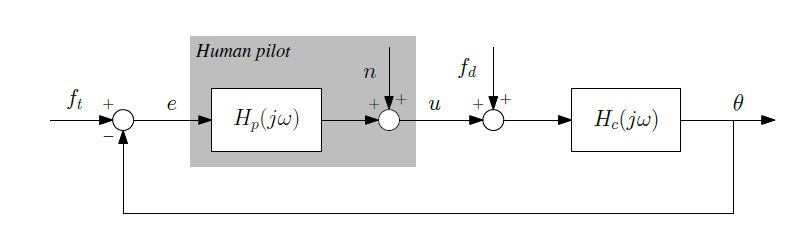
\includegraphics[width = 0.8\linewidth]{images/control_tast.JPG}
\caption{Representation of the compensatory target - following and disturbance-rejection task.}
\label{fig:control task}
\end{figure*}

\subsection{Control variables}
The control variables are kept fixed to prevent biasing and to ensure a fair evaluation. One of the control variables is the control task. In this experiment, a pitch attitude controller task is considered as shown in figure \ref{fig:control task}. The task requires the pilot to follow a target signal, which is combined with a disturbance signal. The objective of the human operator is to make the output of the control element $H_c(jw)$ follow the reference signal with minimal error. The dynamics of the controlled element is given in equation \\\

\begin{equation}
H_{c}(j \omega)=-3.04 \frac{j \omega + 0.99}{j \omega\left((j \omega)^{2}+2.58 j \omega+7.61\right)}
\end{equation}

The manipulator in this case is a side stick to which the control inputs are given. The manipulator should also be the same for all the subjects as changing the environment can lead to biasing and negative outcomes. The display is also a control variable and for tracking the error signal a compensatory. display has been used, as shown in figure \ref{fig:comp disp}.

\begin{figure}[h]
    \centering
    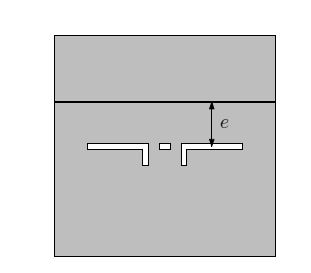
\includegraphics[scale = 1]{images/compensatory.JPG}
    \caption{Compensatory visual display}
    \label{fig:comp disp}
\end{figure}



\subsection{Forcing functions}
To be able to measure the pilot behavior, both a disturbance ($f_d$) and target ($f_t$) forcing function is used. Both signals are (independent) multi-sine forcing functions, consisting of sines with different frequencies. Hence, the forcing functions are in the form as shown in equation \ref{eq:forcingfunctions}.\\

\begin{equation}
\label{eq:forcingfunctions}
f_{d, t}(t)=\sum_{k=1}^{N_{d . t}} A_{d, t}[k] \sin \left(\omega_{d, t}[k] t+\phi_{d, t}[k]\right)
\end{equation}

The disturbance signal $f_d$ is dominant, resulting in a predominantly disturbance-rejection task. To ensure that the participants will not recognize the forcing function, five different realizations of $f_t$ and $f_d$ are varied randomly over trials. Each tracking run lasted 90 seconds. Based on previous experiments \cite{pool2016effects}, only the last 81.92 seconds were used as the measurement data. \\

\subsection{Participants}

The experiment will be using the between-group procedure, the total group of participants consist of sixteen task-naive participants. The subjects for the training will be divided into two groups with eight participant per group. \\

\begin{figure}[h]
    \centering
    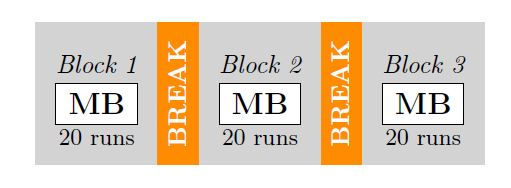
\includegraphics[width = \linewidth]{images/matrix.JPG}
    \caption{Experiment matrix}
    \label{fig:experiment matrix}
\end{figure}

All the participants are asked to perform the same repeated runs of the pitching control task with minor variation to avoid recognition. Each participant will perform 20 tasks repeated over 3 blocks with adequate break in between, thus each participant will do a total of 60 runs. All the participants have to repeat their runs for four consecutive days , such that enough trial data can be collected for evaluation and analysis. In order to keep the participants motivated, at the end of each run feedback about the performance is provided to the participants. This is done by presenting the RMS of the tracking error.\\

%\section{Experiment Data Analysis}

\section{Results}

\subsection{Control behavior and tracking performance}

To validate the relevancy of the hypothesis [\ref{hypothesis 2}] the general trend of the tracking performance and control activity for both the groups over the trial period needs to be analyzed. The optimal method is to fit a learning curve, as described in equation \ref{eq:learning}, through the RMS of each group for tracking task error, control activity and stick deflection respectively. \\

\begin{figure}[h!]
\centering
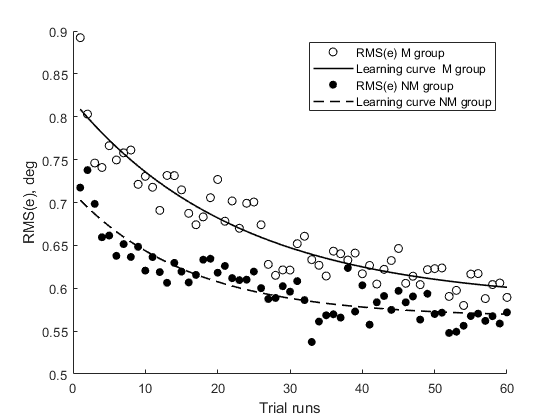
\includegraphics[width = \linewidth]{images/RMS_e.png}
\caption{RMS of tracking error for motion and no motion groups}
\label{fig:RMSerror}
\end{figure}

Figure \ref{fig:RMSerror} visualizes the learning curve for the RMS of the tracking error for both groups. Analytically, it is observed that the initial ($p_0$) and the asymptotic value of error ($p_a$) are higher for the M group compared to the NM. When considering table \ref{NonMotion group learning data} and table \ref{Motion group learning data}, it can be concluded that the learning rate $F$ for the NM group is higher compared to the learning rate of the M group.\\

\begin{figure}[h!]
\centering
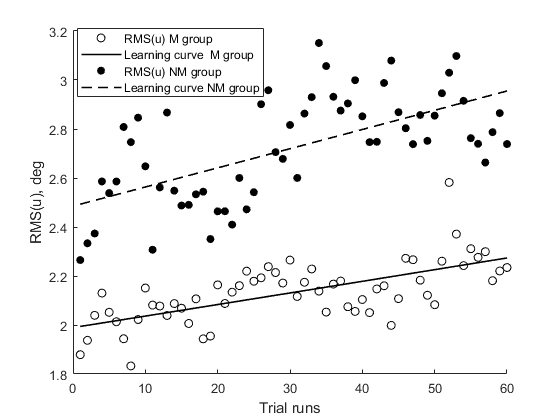
\includegraphics[width = \linewidth]{images/RMS_u.png}
\caption{RMS of control activity for motion and non-motion groups}
\label{fig:RMSu}
\end{figure}

Figure \ref{fig:RMSu} shows that the control activity increases with the number of runs for both groups. The results of the no motion group provide a higher initial and asymptotic value for the control activity compared to the motion group. Again, considering table \ref{NonMotion group learning data} and table \ref{Motion group learning data}, it can be concluded that for the learning rate $F$, the rate for the non-motion group is also significantly higher compared to the motion group. This implies that the no motion group improves their control activity at a faster pace than the motion.\\

\begin{figure}[h!]
\centering
\includegraphics[width = \linewidth]{images/RMS_x.png}
\caption{RMS of stick deflection for motion and no motion groups}
\label{fig:RMSx}
\end{figure}

The final parameter to be analyzed is the stick deflection which is shown in figure \ref{fig:RMSx}. It can be assumed  that better stick movement and control activity can enhance the tracking performance. Better tracking performance implies less tracking task error. The trend of stick deflection is identical to the tracking task error shown in figure \ref{fig:RMSerror}. The $p_0$ value of the curve for the motion group is much higher compared to the non-motion group, so are values for $p_a$. This implies that the motion group provides larger inputs than the non-motion group. When looking at the learning rate $F$ in tables \ref{Motion group learning data} and \ref{NonMotion group learning data}, it can be seen that the curve for no motion group has a steeper rate of change, which indicates that they adjust at a faster rate to the input signals which also in turn results in a higher control activity and less error. \\

\begin{table}[h!]
\centering
\caption{Learning curve model parameter of motion group}
\begin{tabular}{r|r|r|r}
Data & $p_{0_m}\ [deg]$ & $p_{a_m}\ [deg]$ & $F_m\ [-]$\\
\hline
\hline
Tracking error (e) & 0.81883 & 0.5841 & 0.042784\\
Control activity (u)  & 1.9894 & -12.187 & -0.00033094 \\
Stick deflection (x) & 0.9573 & 0.78819 & 0.044666  \\
\end{tabular}
\label{Motion group learning data}
\end{table}

\begin{table}[h!]
\centering
\caption{Learning curve model parameter of no motion group}
\begin{tabular}{r|r|r|r}
Data & $p_{0_{nm}}\ [deg]$ & $p_{a_{nm}}\ [deg]$ & $F_{nm}\ [-]$\\
\hline
\hline
Tracking error (e)  & 0.71167 & 0.56648 & 0.061227 \\
Control activity (u) &  2.4853 & -43.594 & -0.00016907 \\
Stick deflection (x)  & 0.85325 & 0.7724 & 0.084331 \\
\end{tabular}
\label{NonMotion group learning data}
\end{table}


\subsection{Human operator modeling}
In order to see the actual changes in the behavior of the participants, the pilot model as described by equation \ref{eq:pilot model} is fitted to the data of every test run. This is done by setting up a cost function that minimizes the error between the data and the estimated human operator model. This results in a set of optimum values for the different components of the human operator dynamics; $K_p$, $T_L$, $\tau_p$, $\omega_{nm}$, and $\zeta_{nm}$. Example results can be seen in figures \ref{fig:pilotmodel_M} and \ref{fig:pilotmodel_NM}. When looking at these figures, it can already be seen that there is a change in the estimated pilot model. The other participants and other runs show similar results. With this method, the pilot model parameters of every run and every participant can be estimated and the different parameters can be plotted to see the change in behavior with every run. \\

\begin{figure}[h!]
    \centering
    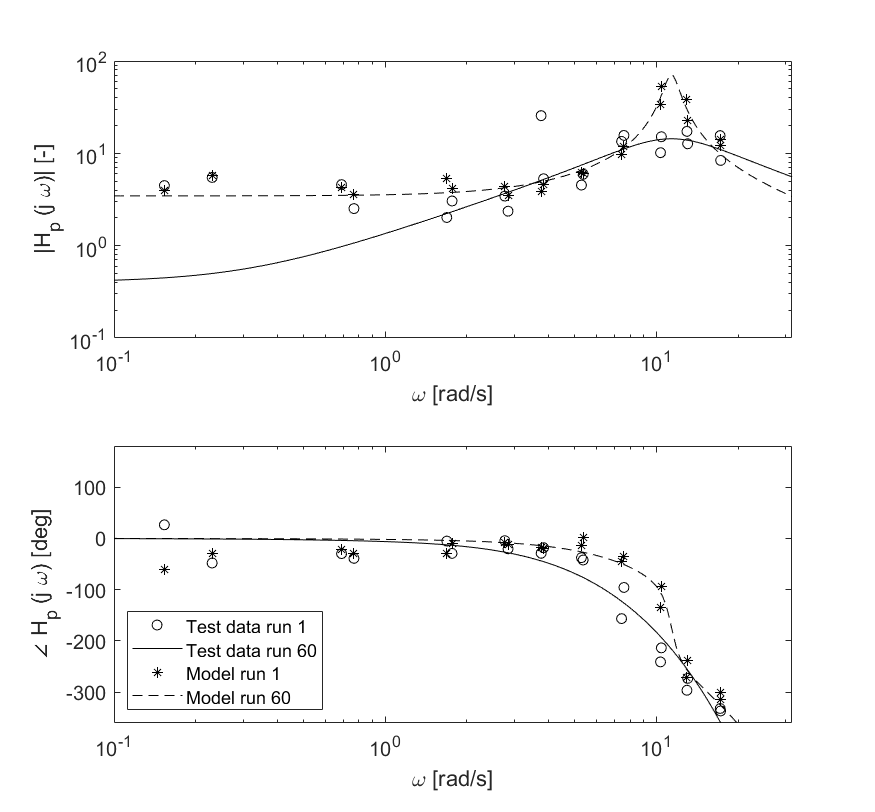
\includegraphics[width=\linewidth]{images/run1_60_participant1M.png}
    \caption{Experiment data and pilot model estimations for run 1 and 60 of participant 8 in group M}
    \label{fig:pilotmodel_M}
\end{figure}


\begin{figure}[h!]
    \centering
    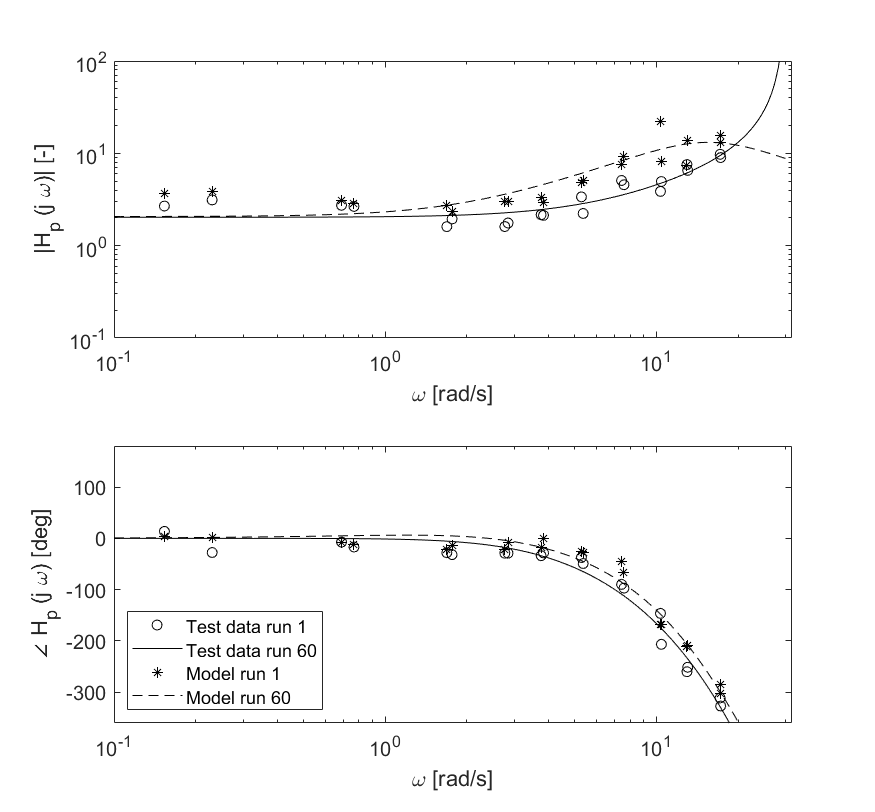
\includegraphics[width=\linewidth]{images/run1_60_participant1NM.png}
    \caption{Experiment data and pilot model estimations for run 1 and 60 of participant 3 in group NM}
    \label{fig:pilotmodel_NM}
\end{figure}

The estimates for all the test runs and all participants can be seen in figure \ref{fig:pilotmodel}. Here, the different parameters $K_p$, $T_L$, $\tau_p$, $\omega_{nm}$, and $\zeta_{nm}$ are plotted against the amount of test runs. In the graphs for the pilot lead/lag time $T_L$, a slight difference between the moving and the non moving simulator groups can be seen and in the neuromuscular damping, a difference can be seen as well. In the neuromuscular natural frequency, almost no difference can be seen. The differences in gain and delay are hidden between the data, so a more zoomed in graph can be seen in figure \ref{fig:zoomed_pilotmodel}. In this figure, the subtle differences between the two groups can be seen. The parameters of the learning curves can  be seen in table \ref{tab:learningcurve_pilot}. \\

\begin{figure*}[h!]
    \centering
    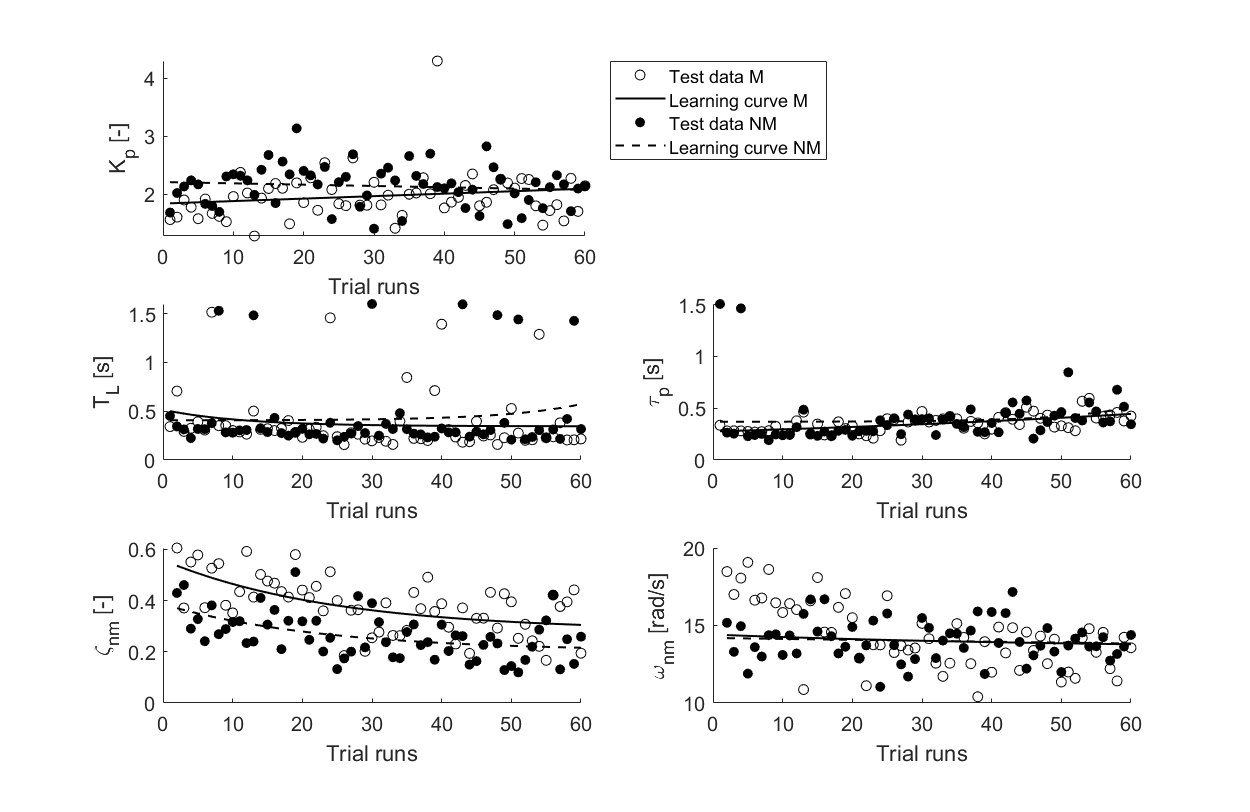
\includegraphics[width=0.9\linewidth]{images/pilot_model2.png}
    \caption{Learning curve of different pilot model parameters}
    \label{fig:pilotmodel}
\end{figure*}


\begin{figure}[h!]
    \centering
    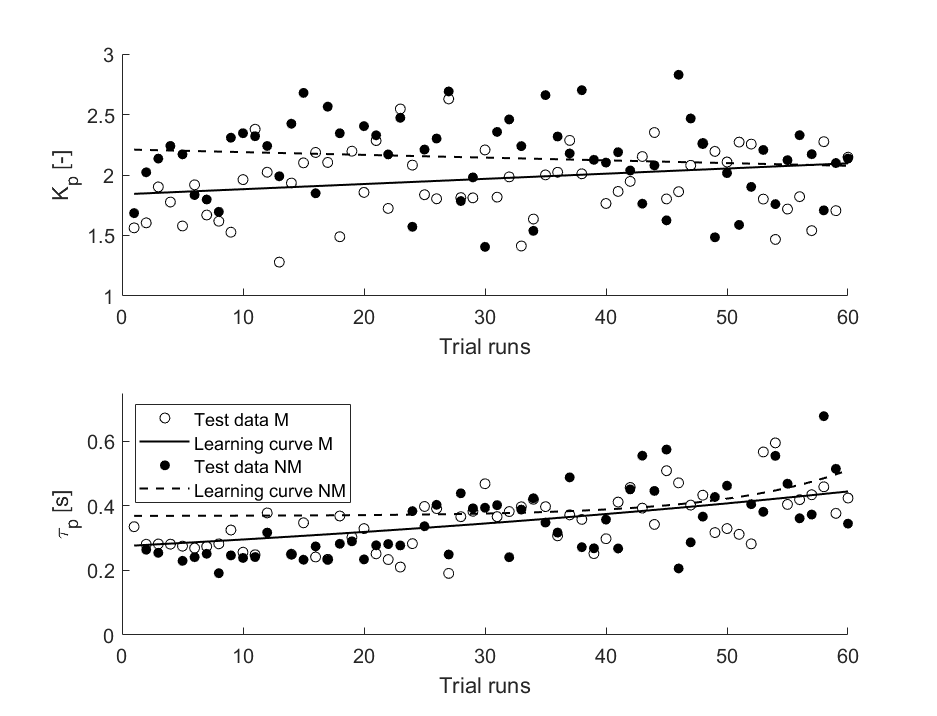
\includegraphics[width=\linewidth]{images/pilot_model_zoomed.png}
    \caption{Zoomed-in graphs for pilot model parameters $K_p$ and $\tau_p$}
    \label{fig:zoomed_pilotmodel}
\end{figure}


\begin{table*}[h!]
\centering
\caption{Learning curve model parameters }
\begin{tabular}{l|c|c|c|c|c|c}
                   & \multicolumn{3}{c|}{\textbf{NM group}} & \multicolumn{3}{c}{\textbf{M group}}                           \\ \hline
\textbf{Parameter} & $F$          & $p_0$     & $p_a$      & $F$           & $p_0$    & $p_a$     \\ \hline\hline
$K_p$              & $8.1419e-05$   & $2.2116$    & $-25.6250$   & $-6.0850e-05$             & $1.8400$                    & -68.2812 \\
$T_L$              & $-0.0942$      & $0.4069$    & $0.4062$     & $0.0833$                  & $0.5149$                    & 0.3455   \\
$\tau_p$           & $-0.1020$      & $0.3691$    & $0.3687$     & $-0.0116$                 & $0.2752$                    & 0.1047   \\
$\zeta_{nm}$       & $0.0425$       & $0.3854$    & $0.2023$     & $0.0403$                  & $0.5580$                    & $0.2815$   \\
$\omega_{nm}$      & $2.1085e-04$   & $14.1953$   & $-14.3750$   & $0.0190$                  & $14.4149$                   & $13.5015$ 
\end{tabular}
\label{tab:learningcurve_pilot}
\end{table*}



\subsection{Statistical test}
\label{sec:statisticaltests} 

The statistical analysis of both the tracking task error and pilot control activity has to be done to determine the validity of \textbf{Hypothesis 2} [\ref{hypothesis 2}]. \textbf{Hypothesis 2} states that there is no notable differences in the performance of no motion and motion groups. The null hypothesis (H=0) suggests that we have enough evidence to accept that the \textbf{Hypothesis 2} and if H = 1, then we can say we don't have enough evidence to accept \textbf{Hypothesis 2} [\ref{hypothesis 2}]. To proceed further, a normality of the pilot error(e) and stick control activity(u) over the last 5 trials. For the normality test for the error and input made by the participants of the two groups the value of H is 0 [table \ref{tab:SWtest}]. H = 0 verifies that the tracking task error and control activity data have a normal distribution. So now to test the validity of the \textbf{Hypothesis 2} we can do a 2 sampled T-test.\\ 

\begin{table*}[!t]
    \centering
    \caption{Shapiro-Wilk normality test for tracking error and control activity}
    \begin{tabular}{c|c|c|c|c|c|c}
    
    Data& $H_m\ [-]$ & $p_m\ [-]$ & $W_m\ [-]$ & $H_{nm\ [-]}$  & $p_{nm}\ [-]$ & $W_{nm}\ [-]$ \\
    \hline
    \hline
    Tracking error(e) & $0$ & $0.8952$ & $0.9732$ & $0$ & $0.2268$ & $0.8598$\\
    Control activity(u) & $0$ & $0.1654$ & $0.8402$ & $0$ & $0.0677$ & $0.7905$\\
    \end{tabular}
    \label{tab:SWtest}
\end{table*}


For T-test the significance value $\alpha$ is set to $0.05$. If the $p$ value is less than $\alpha$ we reject the null hypothesis i.e \textbf{Hypothesis 2} [\ref{hypothesis 2}]. From table \ref{tab:T2test}, we can imply that since the value of H is $1$ and the $p$ values is almost $0$, it is safe to say that we don't have enough evidence statistical to accept the null hypothesis. So in this case the \textbf{Hypothesis 2} is rejected.\\

\begin{table}[ht!]
    \centering
    \caption{Two sampled T-test tracking error and control activity}
    \begin{tabular}{c|c|c}
    Data & $H_t\ [-]$ & $p_t\ [-]$ \\
    \hline
    \hline
    Tracking error (e) & $1$ & $2.8688e-04$\\
    Control activity (u) & $1$ & $5.8148e-04$ \\
    \end{tabular}
    \label{tab:T2test}
\end{table}

One of the criteria for accepting the results from Shapiro-Wilk normality test is to have a high enough $W$ value and the $p$ should be higher than $\alpha$. However, for the input of both the groups and error for the no motion group, the values of $W$ are lower and the $p$ values are higher than $\alpha$, which means that they are not high enough to support the claim of null hypothesis (hypothesis 2 [\ref{hypothesis 2}]) and thus can generate ambiguous results. To cross check the validity of T-test, the Mann-Whitney U test is performed on the two sets of data. The Mann-Whitney U test [table \ref{tab:MWUtest}] shows similar results where not enough evidence is available to accept Hypothesis 2.\\

\begin{table}[!h]
    \centering
    \caption{Mann-Whitney-Wilcoxon test for error and control activity}
    \begin{tabular}{c|c|c}
    Data & $H_w\ [-]$ & $p_w\ [-]$ \\
    \hline
    \hline
    Tracking error(e) & $1$ & $0.0079$\\
    Control Activity(u) & $1$ & $0.0079$ \\
    \end{tabular}
    \label{tab:MWUtest}
\end{table}

So, we can safely say that since H = 1, Hypothesis 2, stating that the two groups will perform the same in the moving base simulator is rejected.

\section{Discussion} 
The goal of this paper is to determine the effectiveness of initial training in a fixed based simulator. The effectiveness is tested by letting task-naive participants perform manual control tasks in a moving simulator.\\

When looking at the first hypothesis \textit{Pilots who received initial fixed-base training will more rapidly acquire manual control skills in a moving-base simulator and will thus, in the early stages of moving-base training, show improved task performance, increased control effort and more “optimal” pilot model parameters compared to pilots who did not receive initial fixed-base training}. In figures \ref{fig:pilotmodel} and \ref{fig:zoomed_pilotmodel}, it is observed that the NM group has a higher initial gain, higher time delays, and higher control activity. Both the higher gains as well as the increased control effort indicated a more ``optimal" pilot; however, the higher time delays indicated the opposite. In figure \ref{fig:zoomed_pilotmodel}, it can be seen that the time delays are relatively close. When looking at the learning rates for the time delays in table \ref{tab:learningcurve_pilot}, it can be seen that the learning rate of the NM group is more negative than that of the M group. So although the initial time delay is worse for the NM group, the learning rate is higher. Further investigation will be needed to fully analyze this, but for now, the pilot model parameters indicate that the NM group with prior fixed-based training do show more optimal pilot behavior in the early stages of the training. \\

When looking at the end of the training runs, the values for $K_p$ and $\tau_p$ seem to converge on each other. However, in figure \ref{fig:RMSu}, there still remains a gap between both groups when looking at the control activity and even a steeper increase in control activity can be observed for the NM group. It is recommended to investigate this in further research. \\

When considering at the RMS of the tracking error it is observed that the M group shows a higher value for the error at the start of the experiment. This was expected since the moving group did not receive initial training. However, the NM group shows a steeper compared to the NM group as can be concluded from table \ref{Motion group learning data} and table \ref{NonMotion group learning data}. Furthermore, it can be observed that after 60 runs the learning curve for the tracking error is almost flat. From this it can be concluded that the participants are fully-learned. Hence a valuable comparison can be made for this between-group experiment. The  RMS data distribution of tracking task error for both the groups have an exponential decay. If the formulation of the learning model[\ref{Dependent variables}] is to be observed, it represents an exponential structure. Thus the data perfectly fits the learning model definition. The learning curve plotted for the tracking task error also represents an exponential decay which matches with the general trend of the data. So it can be concluded that the learning model describes the tracking task error flawlessly.\\

From the RMS of the control activity it can be observed that the value for the NM group is higher compared to the M group. Especially for the NM group, the group averages are deviating from the learning curve quite a lot.  Next to that, even after 60 runs, no flattening of the learning curve is observed. Even though, it was expected to observe fully-learned behavior after 60 runs. This is true for the NM group, as well as for the moving group. Hence, it can be concluded that both groups are not full-learned yet and therefore no good comparison can made regarding the control activity. The no flattening of the learning curve for the control activity could be caused by the mismatch of the control activity data and learning model definition. The trend depicts a continuous increase of the RMS values with a fixed slope. Since the learning model used here in an exponential one, it cannot satisfy the linear nature of the data set. However, since the data is limited here, we cannot fully conclude the fit. A more larger data-set over a prolonged trial period will be helpful here to visualise the trend and fitting the curve. \\

%%question 2 part 1



% stat test discussion
The second hypothesis was defined as: \textit{``After being trained to asymptotic performance in a moving-base simulator, no statistically significant differences in RMS(e) and RMS(u) will exist between pilots who did or did not receive initial fixed-base training."}\\


In section \ref{sec:statisticaltests} it was determined that based on performing two statistical test this hypothesis was rejected. For the error and control activity, we get the value of H as 1, which indicates that we don't have enough evidence to support that the performance of the motion and non-motion group will be same after training. This claim can further be reinforced by figures \ref{fig:RMSerror} and \ref{fig:RMSu} respectively. In figure \ref{fig:RMSerror} for the last 5 runs, it is observed that the RMS(e) of the NM group along the learning curves is approximately below or close to $0.6$, whereas for the motion group  it is close to $0.65$. Similar observations can be made from figure \ref{fig:RMSu}, where the control activity in the last five runs, RMS(u) of the learning curve for the non-motion group is in the range of $2.6 - 2.8$ and on the contrary for the motion group the values lie between $2.0$ and $2.2$. Considering the values for both the error and control activity, it is evident why we get \textbf{H =1} in the statistical test. Thus, we can clearly reject \textbf{Hypothesis 2} stating that a notable difference has been observed between the control activity of the two groups and their performances. Since the NM groups shows a significantly higher control activity and higher learning rate, it can be concluded that the initial training has a positive influence on the performance of the participants.\\


The final hypothesis states \textit{``Essential pilot control behavior parameters for achieving good performance (i.e., $K_p$, $T_L$, and $\tau_p$) will show much clearer learning trends and higher learning rates than pilots’ neuromuscular system parameters (i.e., $\omega_{nm}$ and $\zeta_{nm}$)"}. This hypothesis will be rejected, as the curves in figures \ref{fig:pilotmodel} and \ref{fig:zoomed_pilotmodel} do not show this. For the NM group, the gain and time delays remain fairly constant through the first 40 runs, whereas a clear learning curve is visible for both groups in the neuromuscular damping. In table \ref{tab:learningcurve_pilot}, this is also visible. The learning rate F for both the NM and M group is similar for the neuromuscular damping The neuromuscular frequency shows little to no curve. \\



%Destroy Daan's experiment plan lets go

There are, however, shortcomings in the current way of determining the pilot model parameters. Firstly, the estimates of the pilot model parameters are determined from a cost function, which might not necessarily be the optimal way of determining the parameters. This is due to the cost function being set up without weights, which can lead to overcompensating for one data point which might be an outlier. The effect of this can already be seen in figure \ref{fig:pilotmodel_NM}. In the magnitude plot, the model of the first run shows a large increase towards the right hand side of the graph. Other figures from other participants and other runs sometimes show odd behavior too. This could be prevented by better parameter estimation algorithms or weights in the cost function. One of the benefits of setting up weights is that more weight can be allocated to important parts of the model, for instance around the cross-over frequency. Furthermore, different parameter estimation methods could be implemented in order to make the estimations faster and more accurate.\\


Secondly, the estimated pilot model is not complete. The pilot model as given in equation \ref{eq:pilot model} depicts the lumped pilot model where the true differences in the parameters between the M and NM groups remain hidden. The pilot model for processing motion feedback as well as visual feedback is represented as follows\cite{zaal2009use}: 

\begin{equation}
    H_{p_v} (j \omega) = K_v \frac{(T_{\text{lead}} j \omega + 1)^2}{(T_{\text{lag}} j \omega + 1)} e^{-j \omega \tau_v} H_{nm} (j \omega)
\end{equation}

\begin{equation}
    H_{p_m} (j \omega) = (j \omega)^2 H_{scc} (j \omega) K_m e^{-j \omega \tau_m} H_{nm} (j \omega)
\end{equation}

Where $H_{p_v}$ is the pilot model for the visual feedback and $H_{p_m}$ is the pilot model for the motion feedback. $H_{nm} (j \omega)$ is already defined in equation \ref{eq:neuromuscular} and $H_{scc} (j \omega)$ is defined by Zaal et al \cite{zaal2009modeling}. With these models, the difference in behavior can be attributed to the true parameters that make up the model of the pilot. Setting up the model of the pilot in such a way can lead to a better discussion on the research question and corresponding hypotheses, as a more in-depth view on how the different groups process the vestibular feedback will be available. Next to that, the differences in the motion feedback model can lead to valuable insights on how the fixed-based simulator training can lead to different processing of the input.\\ 

%as the changes in the visual pilot model will become apparent. This can then be compared to the changes in the visual feedback model of the NM group, which will bring us much closer to answering the research question. 


Finally, the amount of participants involved in this research is too little to make statistically sound arguments. Increasing the number of participants will lead to a more general description of pilot behavior and therefore, a more sound comparison between the two different groups will be possible. \\




%%Here explain hypothesis 





%What eects did the prior xed-base training have on tracking performance and control behavior (RMS(e), RMS(u), Kp, TL, p, !nm, nm)? Does this prior training help to learn controlling in a
%moving-base simulator more quickly? And can any dierences observed between training groups be
%proven to be statistically signicant?
%Do you observe dierences in how well the selected learning curve model seems to describe the
%measured data over all experiment trials? Which dependent variables show a more clear learning
%eect than others?
%Do you notice any between-group dierences in your data, even for the nal performed trials, where
%you would expect both groups to be fully learned? What does that imply for the between-comparison
%you are trying to make?





In this part of the discussion, a comparison between two experiment plans will be made. The experiment plan designed by group 1 will be referred to as experiment plan 1 \cite{ref:experimentplan}. The experiment plan provided by the lecturers of AE4316P will be referred to as experiment plan 2 \cite{experimentplan}. Several similarities and differences can be found when considering the two experiment plans. Both experiment plans concern a between-subject training experiment where the influence of using a moving simulator on the training behavior is discussed. In experiment 1, the first group is trained using a non-moving simulator whilst the other group is trained in a moving simulator before evaluation in the moving simulator. In experiment plan 2, only one group is subjected to a training phase in a non-moving simulator before evaluation in the moving simulator. This immediately introduces a difference in the results produced. Furthermore, in experiment plan 1, the participants will perform a small training program to get familiar with the functions in the SIMONA whilst in experiment plan 2 this is not done. \\

%anything chanegd on experiment(more ideas) 
% at least 3 confounds of designed experiment 


Firstly, some changes can be made with respect to communication to the participant. In experiment plan 1, feedback to the participant can be introduced. For instance, an indication of the performance can be communicated to the participant. An example of this would be to show the RMS error value at the end of each run. This can support the motivation of the participant throughout the different runs. Secondly, it would be better to check beforehand if students have experience in flying flight simulators or playing games that might influence performance in the simulator. In addition, it would be better to not train the participants before in knowing the SIMONA since the varying training time influences the results.\\

When performing experiments, it must be noted that confounds can be introduced when performing the experiment. For experiment 1, a confound could be introduced by the mixed expertise of the participants. As proposed in the previous section, before the start of the experiment, questions can be asked about the expertise of the participants, however, these answers are quite subjective. This is defined as a procedural confound. Next to that, the guidelines regarding communication are still quite vague which can also introduce confounds, as different participants may receive different information regarding the experiment. Since working with human participants, the energy and concentration level will highly influence the performance of the participants. For example, if the participant is very tired or not focused, the results of the task performed will not be representative. Part of the focus can be restored by a short break, should the participant indicate that this is necessary. Furthermore, as described before, an indication of the performance can be given to the participants in order to keep the motivation up.\\ %more ideas??nope


When looking at the quality of the answer to research question, it important to emphasize the differences between the research questions. The research question in the first experiment plan focuses on the effect of training in a non-moving simulator in comparison to a moving simulator. In this plan, the value of including a moving simulator in training procedures is investigated. Experiment plan 2 is investigating the influence of prior training in a non-moving simulator compared to having no training at all. Since both research questions are different, no clear comparison can be made between the quality of the experiment set up, since they serve a different goal. However, the research problem is very similar, so one can argue which answer to the research question is most reliable in solving the research problem. In this sense, experiment plan 1 would be more suitable, since in this research a direct comparison between the manual control skill development in a moving and non-moving simulator is made. The answer to this question can directly be used in pilot training to potentially replace expensive training hours in the moving simulator by hours in a non-moving simulator. For experiment plan 2 only the addition of training in a non-moving is investigated. It can potentially lower the amount of time needed in a moving simulator before sufficient skill levels are attained. This can reduce costs, as training in a non-moving simulator is less costly than training in a moving simulator. However, for a direct comparison between the performance of the participants after a moving and non moving simulator, the first experiment plan would be better. \\


For further research some improvements are recommended. Firstly, it is recommended to extend the pilot model. In this paper, no distinction is made between the pilot model for the visual feedback and the motion feedback. To create more detailed analysis two separate pilot models can be introduced to increase the quality of the analysis. Next to that, for this research students are the participants of the experiment. The purpose of this research was to find out if moving simulators could be replaces by non-moving simulator in pilot training. Hence, for further research it is recommended to also perform this experiment with pilots.


\section{Conclusions}
In this paper, the effects of prior fixed-base training on the training of skill-based manual control behavior were evaluated in a compensatory tracking task in a moving-base simulator with 16 task-naive participants. The participants were divided over two groups, where one group did receive prior fixed-base training and the second group did not receive prior training, before training in the moving-base simulator started. To quantify the effects of the prior training, the control behavior of the participants was measured during every run and modeled using a quasi-linear human operator model. The changes in pilot model parameters as well as the tracking error, stick deflection, and control activity were set out against the number of runs, and a exponential learning curve was fitted through the data. 







%\section*{Acknowledgment}


%The authors would like to thank...





% trigger a \newpage just before the given reference
% number - used to balance the columns on the last page
% adjust value as needed - may need to be readjusted if
% the document is modified later
%\IEEEtriggeratref{8}
% The "triggered" command can be changed if desired:
%\IEEEtriggercmd{\enlargethispage{-5in}}

% references section

% can use a bibliography generated by BibTeX as a .bbl file
% BibTeX documentation can be easily obtained at:
% http://www.ctan.org/tex-archive/biblio/bibtex/contrib/doc/
% The IEEEtran BibTeX style support page is at:
% http://www.michaelshell.org/tex/ieeetran/bibtex/
%\bibliographystyle{IEEEtran}
% argument is your BibTeX string definitions and bibliography database(s)
%\bibliography{IEEEabrv,../bib/paper}
%
% <OR> manually copy in the resultant .bbl file
% set second argument of \begin to the number of references
% (used to reserve space for the reference number labels box)
%\begin{thebibliography}{1}

%\bibitem{IEEEhowto:kopka}
%H.~Kopka and P.~W. Daly, \emph{A Guide to \LaTeX}, 3rd~ed.\hskip 1em plus
 % 0.5em minus 0.4em\relax Harlow, England: Addison-Wesley, 1999.
  
%\bibitem{Experimentplangroup1}
%S. Bootsma, T.Mennink, M. Sarkar, \emph{Investigating the influence of motion feedback on manual control skill development during a compensatory tracking task}

%\bibitem{paperzaal}
%Zaal, Peter MT, et al. "Modeling human multimodal perception and control using genetic maximum likelihood estimation." Journal of Guidance, Control, and Dynamics 32.4 (2009): 1089-1099.
%\end{thebibliography}
\bibliographystyle{IEEEtran}
\bibliography{ref}
%\appendix
%\noindent
%\textbf{List of symbols}\\
%$A[k]$ - amplitude of kth sinusoid\\
%$e$ - tracking task error.\\
%$F$ - learning rate.\\
%$f_{d,t}$ - disturbance or reference forcing function \\
%$H_c$ - control element dynamics.\\
%$H_p$ - pilot model transfer function.\\
%$H_{nm}$ - neuromuscular model transfer function.\\
%$H_{scc}$ - semicircular canals model transfer function.\\
%$jw$ - Laplace operator 
%$K$ - gain.\\
%$K_p$ - pilot gain.\\
%$M$ -  moving base simulator group.\\
%$n$ - remnent of the signal.\\
%$n(k)$ - frequency integer factor for kth sinusoid\\
%$NM$ -  fixed based simulator group, then to moving base.\\
%$p_0$ - initial value.\\
%$p_a$ - asymptotic value.\\
%$p$ -  probability.\\
%$R.M.S$ - root mean square.\\
%$T_L$ - pilot lead.\\
%$t$ - time.\\
%$u$ - control input.\\
%$W$ - weight of test.\\
%$x$ - stick deflection.\\
%$y_t$ - target signal.\\
%$y_d$ - disturbance or noise.\\
%$y(x)$  - learning curve model.\\
%\newline
%$\alpha$- Significance value , 0.05.\\
%$\omega$ - frequency \\
%$\omega_{nm}$ - frequency of neuromuscular activity.\\
%$\phi$ - phase delay.\\
%$\tau$ - time delay constant.\\
%$\tau_p$ - pilot time delays \\
%$\zeta_{nm}$ - neuromuscular damping ratio.\\

%\newline
%\noindent 
%\textbf{Subscripts} \\
%\noindent $m$ - Motion feedback system \\
%$v$ - Visual feedback system

% that's all folks
\end{document}


